%% ----------------------------------------------------------------
%% Thesis.tex -- MAIN FILE 
%% ---------------------------------------------------------------- 

% Set up the document
\documentclass[a4paper, 11pt, oneside]{Thesis}  % Use the "Thesis" style, based on the ECS Thesis style by Steve Gunn
\graphicspath{Figures/}  % Location of the graphics files (set up for graphics to be in PDF format)
% Table configuration packages
\usepackage{array,graphicx}
\usepackage{booktabs}
\usepackage{pifont}
\usepackage{libertine}
\usepackage{tabu}
\usepackage{longtable}
\usepackage[table]{xcolor}
\usepackage{tcolorbox}
\usepackage{textcomp}
\usepackage{multicol}
% My additions
\usepackage{amsmath}
\usepackage[utf8]{inputenc}
\usepackage{pgfplots}
\usepackage{tikz}
\usepackage[outline]{contour} % glow around text
\usepackage{listofitems} % for \readlist to create arrays
\usepackage{bm}


\DeclareUnicodeCharacter{2212}{−}
\usepgfplotslibrary{groupplots,dateplot}
\usetikzlibrary{patterns,shapes.arrows}
\pgfplotsset{compat=newest}
% \usepackage[table,xcdraw]{xcolor}
% \newtheorem{definition}{Definition}
%

\makeatother

% Include any extra LaTeX packages required
\usepackage[square, numbers, comma, sort&compress]{natbib}  % Use the "Natbib" style for the references in the Bibliography
\usepackage{verbatim}  % Needed for the "comment" environment to make LaTeX comments
\usepackage{float} % To keep figures in place
\hypersetup{urlcolor=black, colorlinks=false, pdfborder = {0 0 0}}  % Colours hyperlinks in blue
% Define enumerated description lists
\usepackage{enumitem}
\newcounter{descriptcount}
\newcounter{descriptcount2}
\newlist{enumdescript}{description}{2}
\setlist[enumdescript,1]{%
  before={\setcounter{descriptcount}{0}%
          \renewcommand*\thedescriptcount{\arabic{descriptcount}.}}
  ,font=\bfseries\stepcounter{descriptcount}\thedescriptcount~
}
\setlist[enumdescript,2]{%
  before={\setcounter{descriptcount2}{0}%
          \renewcommand*\thedescriptcount{\roman{descriptcount2}.}}
  ,font=\bfseries\stepcounter{descriptcount2}\thedescriptcount~
}
 

 
%% ----------------------------------------------------------------
\begin{document}

% For changes in supervisor, degree type, research group, etc. please change the Thesis.cls file
\frontmatter      % Begin the book's numbering; frontpage
%
%\pagenumbering{arabic}

% Set up the Title Page
\title  {Thesis Title}

\authors  {\texorpdfstring
            {\href{mailto:itsouros@auth.gr}{Iakovos Marios Tsouros}}
            {Author's Name}
            }
\addresses  {\groupname\\\deptname\\\univname}  % Do not change this here, instead these must be set in the "Thesis.cls" file, please look through it instead
\date       {Date}
\subject    {}
\keywords   {}

\maketitle

%% ----------------------------------------------------------------

\setstretch{1.3}  % It is better to have smaller font and larger line spacing than the other way round

% Define the page headers using the FancyHdr package and set up for one-sided printing
\fancyhead{}  % Clears all page headers and footers
\rhead{\thepage}  % Sets the right side header to show the page number
\lhead{}  % Clears the left side page header

\pagestyle{fancy}  % Finally, use the "fancy" page style to implement the FancyHdr headers

%% ----------------------------------------------------------------
% Declaration Page required for the Thesis, your institution may give you a different text to place here
\Declaration{

\addtocontents{toc}{\vspace{1em}}  % Add a gap in the Contents, for aesthetics

I, [author's name], declare that this thesis titled, [thesis title] and the work presented in it are my own. I confirm that:

\begin{itemize} 
\item[\tiny{$\blacksquare$}] This work was done wholly or mainly while in candidature for a research degree at this University.
 
\item[\tiny{$\blacksquare$}] Where any part of this thesis has previously been submitted for a degree or any other qualification at this University or any other institution, this has been clearly stated.
 
\item[\tiny{$\blacksquare$}] Where I have consulted the published work of others, this is always clearly attributed.
 
\item[\tiny{$\blacksquare$}] Where I have quoted from the work of others, the source is always given. With the exception of such quotations, this thesis is entirely my own work.
 
\item[\tiny{$\blacksquare$}] I have acknowledged all main sources of help.
 
\item[\tiny{$\blacksquare$}] Where the thesis is based on work done by myself jointly with others, I have made clear exactly what was done by others and what I have contributed myself.
\\
\end{itemize}
 
 
Signed:\\
\rule[1em]{25em}{0.5pt}  % This prints a line for the signature
 
Date:\\
\rule[1em]{25em}{0.5pt}  % This prints a line to write the date
}
\clearpage  % Declaration ended, now start a new page

%% ----------------------------------------------------------------
% The "Funny Quote Page"
\pagestyle{empty}  % No headers or footers for the following pages

\null\vfill
% Now comes the "Funny Quote", written in italics
\textit{Inspiring quote goes here (optional)}

\begin{flushright}
Quote's attribution
\end{flushright}

\vfill\vfill\vfill\vfill\vfill\vfill\null
\clearpage  % Funny Quote page ended, start a new page
%% ----------------------------------------------------------------

% The Abstract Page
\addtotoc{Abstract}  % Add the "Abstract" page entry to the Contents
\abstract{
\addtocontents{toc}{\vspace{1em}}  % Add a gap in the Contents, for aesthetics

Abstract goes here.

}

\clearpage  % Abstract ended, start a new page
%% ----------------------------------------------------------------

\setstretch{1.3}  % Reset the line-spacing to 1.3 for body text (if it has changed)

% The Acknowledgements page, for thanking everyone
\acknowledgements{
\addtocontents{toc}{\vspace{1em}}  % Add a gap in the Contents, for aesthetics
Acknowledgements go here.

}
\clearpage  % End of the Acknowledgements
%% ----------------------------------------------------------------

\pagestyle{fancy}  %The page style headers have been "empty" all this time, now use the "fancy" headers as defined before to bring them back


%% ----------------------------------------------------------------
\lhead{\emph{Contents}}  % Set the left side page header to "Contents"
\tableofcontents  % Write out the Table of Contents

%% ----------------------------------------------------------------
\lhead{\emph{List of Figures}}  % Set the left side page header to "List if Figures"
\listoffigures  % Write out the List of Figures

%% ----------------------------------------------------------------
\lhead{\emph{List of Tables}}  % Set the left side page header to "List of Tables"
\listoftables  % Write out the List of Tables

%% ----------------------------------------------------------------
\setstretch{1.5}  % Set the line spacing to 1.5, this makes the following tables easier to read
\clearpage  % Start a new page
\lhead{\emph{Abbreviations}}  % Set the left side page header to "Abbreviations"
\listofsymbols{ll}  % Include a list of Abbreviations (a table of two columns)
{
\textbf{Acronym} & \textbf{W}hat (it) \textbf{S}tands \textbf{F}or \\
% Abbreviations go here
}

\lhead{}
%% ----------------------------------------------------------------
% End of the pre-able, contents and lists of things
% Begin the Dedication page

\setstretch{1.3}  % Return the line spacing back to 1.3

\pagestyle{empty}  % Page style needs to be empty for this page
\dedicatory{Dedication (optional)}

\addtocontents{toc}{\vspace{2em}}  % Add a gap in the Contents, for aesthetics


%% ----------------------------------------------------------------
\mainmatter	  % Begin normal, numeric (1,2,3...) page numbering
\pagestyle{fancy}  % Return the page headers back to the "fancy" style

% Include the chapters of the thesis, as separate files
% Just uncomment the lines as you write the chapters

\chapter{Introduction} \label{introduction}
\graphicspath{Figures/chapter1/}
\section{Graphs}
In this subsection, the main aspects of graph theory are briefly presented.
\subsection{Introduction}


% \subsubsection{Begginings and historical remarks}


% \subsubsection{Introduction}

In the real world, many problems can be described by a diagram connecting a set of points with
lines, joining pairs of these points, or even creating loops on a single point. A simple example
of that would be a set of points representing people with lines connecting acquintances, or
points representing atoms and lines representing chemical bonds, creating a representation of
a molecule as a graph attribute. In the examples above, the only information contained is whether
two points are associated, with the manner being disregarded. The concept of a graph consists of
a mathematical abstraction of the above. \cite{book:2008}


\begin{definition} \label{u_simple_graph} Mathematically, in its simplest form, a
  \textbf{graph} is an ordered pair\footnotemark{} $G=(V, E)$ of:
  \begin{itemize}
  \item \textbf{V}, a set of vertices (also known as nodes).
  \item $E \subseteq \{\{x, y\} | x,y \in V ~x \neq y \}$, which is the set of \textbf{edges}
    which consists of unordered pairs of vertices that connect two nodes.
  \end{itemize}
\footnotetext{An ordered pair $(a, b)$ is a pair of objects in which the order of
appearance or insertion is significant; the ordered pair $(a, b)$ is different than $(b,
a)$ unless $a=b$. An unordered pair is a set of the form ${a, b}$ is a set having two
elements with no relation between them and ${a, b} = {b, a}$.  }
\end{definition}

This type of object is called an \textbf{undirected simple graph} to avoid confusion
with other types.

\begin{definition}\label{graph_def}
  A \textit{graph} G is an ordered pair $(V(G), E(G))$ consisting of a set
$V(G)$ of \textit{vertices} (also called \textit{nodes} or \textit{points}) and a set
$E(G)$, disjoint from $V(G)$ which consists of \textit{edges} (also called \textit{links}
or \textit{lines}) together with an incidence function $\psi_G$ that associates with each
edge of G an unordered pair of not necesserily distinct vertices of G.  If $e$ is an edge
and $u$ and $v$ are vertices such that $\psi_G ={u, v}$ then $e$ is said to \textit{join}
$u$ and $v$, and the vertices $u$ and $v$ are called the \textit{ends} of $e$. We denote
the numbers of vertices and edges $G$ by $u(G)$ and $e(G)$ which two parameters are called
the \textit{order} and \textit{size} of G, respectively \cite{book:2008}.

  In short, we can define a \textbf{graph} as an ordered triple $G=(V, E, \phi_G)$
consisting of:
  \begin{itemize}
  \item $V$, a set of \textit{vertices}
  \item $E$, a set of \textit{edges}
  \item $\phi_G: E \rightarrow \{\{x, y\} | x, y \in V \; and \; x \neq y\}$ an
\textit{incidence function} mapping every edge to an unordered pair of vertices - an edge
associated with two distinct vertices. The incidence function is a function of the edges.
  \end{itemize} This type of object is called an \textit{undirected multigraph}, to avoid
confusion. Note, that the above definition of the \textit{incidence function} does not
allow for \textit{loops} (mappings of an edge on the same vertex).

A \textit{loop} is a an edge that allows a connection of a vertex to itself and a graph can
be defined to either allow or disallow the presence of loops. Some authors allow for loops
to exist on \textit{multigraphs} \cite{article:bollobas}, while other consider these kind
of graphs to exist in a different category, called \textit{pseudographs} \cite{book:Gary}.
Allowing loops requires modifying the incidence function so they can be supported. The new
incidence function can be written as:
\begin{equation}\label{eq:phi} \phi_G : E \rightarrow \{\{x, y \} | x,y \in V\} \end{equation}
The example presented below should better illustrate clarify the definition (of a pseudograph).
\begin{figure}[H]
  \begin{center}
  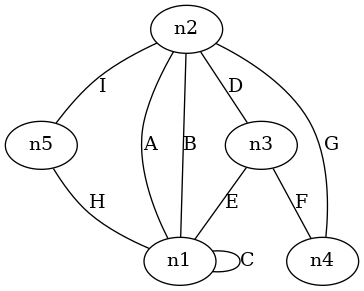
\includegraphics[scale=0.5]{Figures/chapter1/definition_ex_1.png}
\end{center}
  \caption{An undirected pseudograph with labeled nodes and
edges.}\label{fig:SimplePseudograph}

\end{figure}
\begin{example}

  \

For the graph presented in  \fref{fig:SimplePseudograph}  the following
can be assumed:
\begin{align*}
    &G = (V(G), E(G))
    &\intertext{and} 
    &V(G) = \{n_1, n_2, n_3, n_4, n_5\} \\
    &E(G) = \{A, B, C, D, E, F, G, H, I\} 
    &\intertext{and the incidence function is defined as:}
    &\psi_G(A) = n_1n_2,\quad \psi_G(B) = n_1n_2, \quad \psi_G(C) =
      n_1n_1, \quad \psi_G(D) = n_2n_3,\\
    &\psi_G(E) = n_1n_3, \quad \psi_G(F) = n_3n_4, \quad \psi_G(G) = n_2n_4,
      \quad \psi_G(H)= n_1n_5, \\
    &\psi_G(I) = n_2n_5
\end{align*}
\end{example}
  
It should now be clear that with the newer definition of $\phi_G$, self loops are now possible.
Additionaly, even though this was not prohibited by the previous definition, it is worth
noting that a node can be connected to another with multiple edges (or multiedges), or that it can have zero
connections to other nodes. Generally, $V$ is assumed to be a non-empty set, but $E$ can be
empty.

It is now possible to define some characteristic attributes of graphs:
\begin{itemize}
\item $|V|$: the \textbf{order} of a graph is the number of its vertices.
\item $|E|$: the \textbf{size} of a graph is the number of its edges.
\item The \textbf{degree} (or \textbf{valency}) of a single node is the number of
  edges connected to it. The \textbf{degree} of a graph is the maximum number of
  edges connected to a single vertex that belongs to it.
\item The edges of create a \textit{homogenous relation}\footnotemark{} $\sim$ on the vertices
  of the graph that is called \textbf{adjacency relation}; for each edge \textit{$(x, y)$}, its
  endpoints \textit{x, y} are said to be \textbf{adjacent} to each other, denoted by $x \sim y$.
  This property will be particulary useful when the adjacency matrix is defined in the following
  section.
\end{itemize}

\footnotetext{A \textbf{homogenous relation} (or \textbf{endorelation}) over a set \textit{X}
  is a set of assignments (binary relations) over \textit{X} and itself; i.e. it is a subset of
  the cartesian product $X\times X$
}

It can be inferred from the above definitions and attributes that for an undirected
graph of order \textit{n}, the maximum \textit{degree} of a node is $n~-~1$ and
and maximum \textit{size} of a graph is $n(n~-~1)/2$.

\end{definition}

In this section only \textit{undirected} graphs were considered, which are graphs
with edges with no orientation. A whole other class of graph objects with edges which
have orientation exists, called \textit{directed graphs}. These kind of graphs objects
are out of scope for this thesis and will not be presented.


\subsection{Adjacency Matrix}
\begin{definition}
  The \textit{adjacency matrix} is the fundamental mathematical representation of a graph.
  It is a square matrix, the elements of which represent which pair of nodes are
  \textit{adjacent} or not. Thus, the adjacency matrix \textbf{A} of a graph of order $n$
  is the $n\times n$ matrix with elements $A_{ij}$ such that:
  \begin{equation}
    \label{eq:adj_mat}
    A_{ij} = \begin{cases} 1 &\text{if there exists at least one edge connecting $i$ and $j$} \\
               0 &\text{if there no edges connecting those edges directly.}

             \end{cases}
\end{equation}
\end{definition}


\begin{figure}
     \begin{subfigure}[t]{0.4\textwidth}
         \centering
         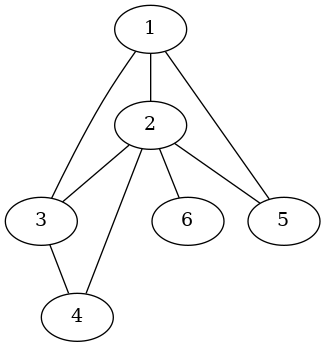
\includegraphics[width=\textwidth]{Figures/chapter1/simple_graph_adj.png}
         \caption{Multigraph with no loops and multiple edges.}
         \label{fig:simple_adj_demo}
     \end{subfigure}
     \hfill
     \begin{subfigure}[t]{0.4\textwidth}
         \centering
         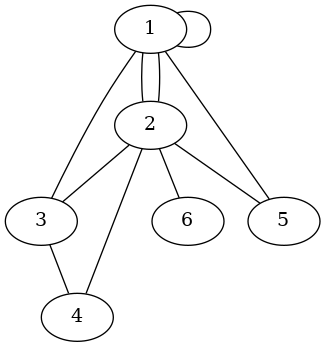
\includegraphics[width=\textwidth]{Figures/chapter1/complex_graph_adj.png}
         \caption{Mutligraph with loops and multiple edges.}
         \label{fig:compl_adj_demo}
     \end{subfigure}
        \caption{Two undirected multigraphs.}
        \label{fig:two multigraphs}
\end{figure}

Considering the simple undirected graph of \fref{fig:simple_adj_demo} we can construct
the following adjacency matrix:
\begin{table}[H]
  
  \begin{equation*}
    A = 
    \begin{pmatrix}
      0 & 1 & 1 & 0 & 1 & 0 \\
      1 & 0 & 1 & 1 & 1 & 1 \\
      1 & 1 & 0 & 1 & 0 & 0 \\
      0 & 1 & 1 & 0 & 0 & 0 \\
      1 & 1 & 0 & 0 & 0 & 0 \\
      0 & 1 & 0 & 0 & 0 & 0 
    \end{pmatrix}
  \end{equation*}
  \caption{Adjacency matrix for \fref{fig:simple_adj_demo}}
\end{table}

For this simple network, which has no loops and only one edge connect two nodes,
the diagonal matrix elements are always zero and the matrix is symmetric, as for
each edge connecting $i$ and $j$ there is a representation for the $j$ to $i$ connection
as well.

In a more complex case, such as the one presented in \fref{fig:compl_adj_demo} where loops
and multiedges are present an adjacency matrix can still be constructed. In this case,
a multiedge is represented by setting the value of the corresponding $A_{ij}$ value equal
to the multiplicity of the edge. In this case, $A_{12} = A_{21} = 2$.

For loops, the most common representation in the case of undirected
graphs is to still set the value of the $A_{ii}$ element equal to $2$
(i.e. $A_{11} = 2$ in the example presented).  Essentially, an edge of
a loop has two ends that connect to the same node, thus the result
\cite[p.~68]{book:algebraic}. Additionaly, defining the matrix in such
manner, allows for better computations and is consistent with the
definition of the representation of an edge connecting two nodes of an
undirected graph \cite[p.~108]{book:Newman}. 

Thus, the adjacency matrix for the graph of \fref{fig:compl_adj_demo} is

\begin{table}[H]
  \begin{equation*}
    A = 
   \begin{pmatrix}
      2 & 2 & 1 & 0 & 1 & 0 \\
      2 & 0 & 1 & 1 & 1 & 1 \\
      1 & 1 & 0 & 1 & 0 & 0 \\
      0 & 1 & 1 & 0 & 0 & 0 \\
      1 & 1 & 0 & 0 & 0 & 0 \\
      0 & 1 & 0 & 0 & 0 & 0 
    \end{pmatrix}
  \end{equation*}
  \caption{Adjacency matrix for  \fref{fig:compl_adj_demo}}
\end{table}
 % Introduction

\chapter{Neural Networks} \label{literature}

% \section{Background - Artificial Neural Networks}

% \subsection{Introduction}

\section{Historical Background}

\textbf{Artificial Neural Networks (ANN)}, or sometimes simply called
\textbf{neural networks} is a class of computational models that mimic
the way biological neural networks work, such as the human brain. Interest
on the subject sparked after the seminal paper \textit{"A Logical
Calculus of the Ideas Immanent in Nervous Activity"}
\cite{article:McCulloch1943} by Warren McCulloch and Walter Pitts, where
they proposed a computationally functional model of neural networks.
Their suggestions showed that in principle, any function a digital computer
can compute, a neural net should too. The models they described had weights
and thresholds, but they lacked a training method. 

The suggestions of McCulloch and Pitts lead Frank Rosenblatt to create
the \textit{Perceptron} in 1958 \cite{article:Rosenblatt1958ThePA}, a
binary classifier algorithm based on supervised
learning\footnote{Supervised learning is a machine learning training
technique that optimizes a model based on examples input-output
pairs.}. Although initially promising, single layer perceptrons were
not able to train on multiple classes of patterns and were eventually
proven incapable of learning a XOR function \footnote{XOR (Exclusive
or, $x\oplus y$) is a logical operation that is true only if its
arguments differ.} in the book \textit{Perceptrons}
\cite{book:minsky1969perceptrons}, as the way they worked was by
``separating'' data linearly. This lead to a stagnation in machine
learning research dubbed ``AI winter'', until the proposal of
\textbf{backpropagation\footnote{Backpropagation is a method of fine
tuning a neural network based on the error rate obtained from previous
runs of the program. It will be discussed in detail later in this
thesis.}} by Paul John Werbos in 1975 \cite{book:werbos1975beyond}.

A renewed interest in the field lead to the development of the
Cresceptron \cite{article:Cresceptron} in 1992, a method of training
large networks with pooling layers (\textbf{max-pooling}) and down-sampling.
GPU\footnote{GPU - Graphics Processing Units is a specialized
electronic circuit, a central part of modern computers which excels in
    efficient computation of algorithms which process large blocks of data
    parallelly, thus exceling in machine learning applications.} usage made
    possible the training of larger networks, while new types of networks
    emerged such as the \textbf{Recurrent Neural Networks (RNNs)}.
    \textbf{Convolutional Neural Networks} have recently proven to be
    far superior for image classification tasks.

    In recent years, neural 


    \subsection{Basics}
    \subsubsection{Summary}

    One can think of ANNs as a directed graph, with a collection of nodes
    which are densely connected (called \textbf{artificial neurons}),
    transimiting signals to each other. These nodes are usually organized
    in sets of layers, with signals moving in one direction
    (i.e. \textit{feed forward networks}) through weighted connections.
    Signals received on a single neuron are real numbers, and the output
    of a single neuron is the output of an aggregation of a non-linear
    function of the sum of its inputs. This function is called an
    \textit{activation function} and its results are propagated to all of
    the nodes outgoing connections.  Thus, each neuron can be thought as a
    simple processing unit. The weighted connections between nodes might
    have an excitatory or inhibitory effect, based on these weights which
    can be positive, negative or very close to zero, having no effect
    \cite[Chap. ~ 1]{book:Gurney1997AnIT}. While training, example
    data is passed through the input layer and gets radically transformed
    through the layers until it reaches the output layer. The weights and
    other trainable parameters are then adjusted until the training data
    consistently reaches satisfactory results.

    \begin{figure}[h!]
    \centering
    % % \documentclass[tikz]{standalone}
% \usepackage{tikz}
    \usetikzlibrary{positioning}

\tikzset{basic/.style={draw,fill=blue!50!green!20,text width=1em,text badly centered}}
\tikzset{input/.style={basic,circle}}
\tikzset{weights/.style={basic,rectangle}}
\tikzset{functions/.style={basic,circle,fill=blue!10}}

% \begin{document}
    \begin{tikzpicture}
        \node[functions] (center) {};
        \node[below of=center,font=\scriptsize,text width=4em] {Activation function};
        \draw[thick] (0.5em,0.5em) -- (0,0.5em) -- (0,-0.5em) -- (-0.5em,-0.5em);
        \draw (0em,0.75em) -- (0em,-0.75em);
        \draw (0.75em,0em) -- (-0.75em,0em);
        \node[right of=center] (right) {};
            \path[draw,->] (center) -- (right);
        \node[functions,left=3em of center] (left) {$\sum$};
            \path[draw,->] (left) -- (center);
        \node[weights,left=3em of left] (2) {$w_2$} -- (2) node[input,left of=2] (l2) {$x_2$};
            \path[draw,->] (l2) -- (2);
            \path[draw,->] (2) -- (left);
        \node[below of=2] (dots) {$\vdots$} -- (dots) node[left of=dots] (ldots) {$\vdots$};
        \node[weights,below of=dots] (n) {$w_n$} -- (n) node[input,left of=n] (ln) {$x_n$};
            \path[draw,->] (ln) -- (n);
            \path[draw,->] (n) -- (left);
        \node[weights,above of=2] (1) {$w_1$} -- (1) node[input,left of=1] (l1) {$x_1$};
            \path[draw,->] (l1) -- (1);
            \path[draw,->] (1) -- (left);
        \node[weights,above of=1] (0) {$w_0$} -- (0) node[input,left of=0] (l0) {$1$};
            \path[draw,->] (l0) -- (0);
            \path[draw,->] (0) -- (left);
        \node[below of=ln,font=\scriptsize] {inputs};
        \node[below of=n,font=\scriptsize] {weights};
    \end{tikzpicture}
% \end{document}
    \scalebox{.8}{% See https://tikz.net/neural_networks/ for more.
\usetikzlibrary{arrows.meta} % for arrow size
\contourlength{1.4pt}
\tikzset{>=latex} % for LaTeX arrow head
% \usepackage{xcolor}
\colorlet{myred}{red!80!black}
\colorlet{myblue}{blue!80!black}
\colorlet{mygreen}{green!60!black}
\colorlet{myorange}{orange!70!red!60!black}
\colorlet{mydarkred}{red!30!black}
\colorlet{mydarkblue}{blue!40!black}
\colorlet{mydarkgreen}{green!30!black}
\tikzstyle{node}=[thick,circle,draw=myblue,minimum size=22,inner sep=0.5,outer sep=0.6]
\tikzstyle{node in}=[node,green!20!black,draw=mygreen!30!black,fill=mygreen!25]
\tikzstyle{node hidden}=[node,blue!20!black,draw=myblue!30!black,fill=myblue!20]
\tikzstyle{node convol}=[node,orange!20!black,draw=myorange!30!black,fill=myorange!20]
\tikzstyle{node out}=[node,red!20!black,draw=myred!30!black,fill=myred!20]
\tikzstyle{connect}=[thick,mydarkblue] %,line cap=round
\tikzstyle{connect arrow}=[-{Latex[length=4,width=3.5]},thick,mydarkblue,shorten <=0.5,shorten >=1]
\tikzset{ % node styles, numbered for easy mapping with \nstyle
  node 1/.style={node in},
  node 2/.style={node hidden},
  node 3/.style={node out},
}
\def\nstyle{int(\lay<\Nnodlen?min(2,\lay):3)} % map layer number onto 1, 2, or 3
\begin{tikzpicture}[x=2.2cm,y=1.4cm]
  \message{^^JNeural network, shifted}
  \readlist\Nnod{4,5,3} % array of number of nodes per layer
  \readlist\Nstr{n,m,k} % array of string number of nodes per layer
  \readlist\Cstr{\strut x,a^{(\prev)},y} % array of coefficient symbol per layer
  \def\yshift{0.5} % shift last node for dots
  
  \message{^^J  Layer}
  \foreachitem \N \in \Nnod{ % loop over layers
    \def\lay{\Ncnt} % alias of index of current layer
    \pgfmathsetmacro\prev{int(\Ncnt-1)} % number of previous layer
    \message{\lay,}
    \foreach \i [evaluate={\c=int(\i==\N); \y=\N/2-\i-\c*\yshift;
                 \index=(\i<\N?int(\i):"\Nstr[\lay]");
                 \x=\lay; \n=\nstyle;}] in {1,...,\N}{ % loop over nodes
      % NODES
      \node[node \n] (N\lay-\i) at (\x,\y) {$\Cstr[\lay]_{\index}$};
      
      % CONNECTIONS
      \ifnum\lay>1 % connect to previous layer
        \foreach \j in {1,...,\Nnod[\prev]}{ % loop over nodes in previous layer
          \draw[connect,white,line width=1.2] (N\prev-\j) -- (N\lay-\i);
          \draw[connect arrow] (N\prev-\j) -- (N\lay-\i);
          % \draw[connect] (N\prev-\j) -- (N\lay-\i)
          %    node[pos=0.50] {\contour{white}{$w_{1, \index}$}};
          %\draw[connect] (N\prev-\j.0) -- (N\lay-\i.180); % connect to left
        }
      \fi % else: nothing to connect first layer
      
    }
    \path (N\lay-\N) --++ (0,1+\yshift) node[midway,scale=1.5] {$\vdots$};
  }
  
  % LABELS
  \node[above=5,align=center,mygreen!60!black] at (N1-1.90) {input\\[-0.2em]layer};
  \node[above=2,align=center,myblue!60!black] at (N2-1.90) {hidden layer};
  \node[above=10,align=center,myred!60!black] at (N\Nnodlen-1.90) {output\\[-0.2em]layer};
  
\end{tikzpicture}}
    \caption{A simple neural network demonstrating the layered structure and
    and flow of data from input to output.}
    \label{fig:simple_nn_demo}
    \end{figure}
    \newpage
    % \section{Backpropagation}
    \subsubsection{Building Blocks}
    % \begin{figure}[t!]
    %   \centering
    %   % % \documentclass[tikz]{standalone}
% \usepackage{tikz}
    \usetikzlibrary{positioning}

\tikzset{basic/.style={draw,fill=blue!50!green!20,text width=1em,text badly centered}}
\tikzset{input/.style={basic,circle}}
\tikzset{weights/.style={basic,rectangle}}
\tikzset{functions/.style={basic,circle,fill=blue!10}}

% \begin{document}
    \begin{tikzpicture}
        \node[functions] (center) {};
        \node[below of=center,font=\scriptsize,text width=4em] {Activation function};
        \draw[thick] (0.5em,0.5em) -- (0,0.5em) -- (0,-0.5em) -- (-0.5em,-0.5em);
        \draw (0em,0.75em) -- (0em,-0.75em);
        \draw (0.75em,0em) -- (-0.75em,0em);
        \node[right of=center] (right) {};
            \path[draw,->] (center) -- (right);
        \node[functions,left=3em of center] (left) {$\sum$};
            \path[draw,->] (left) -- (center);
        \node[weights,left=3em of left] (2) {$w_2$} -- (2) node[input,left of=2] (l2) {$x_2$};
            \path[draw,->] (l2) -- (2);
            \path[draw,->] (2) -- (left);
        \node[below of=2] (dots) {$\vdots$} -- (dots) node[left of=dots] (ldots) {$\vdots$};
        \node[weights,below of=dots] (n) {$w_n$} -- (n) node[input,left of=n] (ln) {$x_n$};
            \path[draw,->] (ln) -- (n);
            \path[draw,->] (n) -- (left);
        \node[weights,above of=2] (1) {$w_1$} -- (1) node[input,left of=1] (l1) {$x_1$};
            \path[draw,->] (l1) -- (1);
            \path[draw,->] (1) -- (left);
        \node[weights,above of=1] (0) {$w_0$} -- (0) node[input,left of=0] (l0) {$1$};
            \path[draw,->] (l0) -- (0);
            \path[draw,->] (0) -- (left);
        \node[below of=ln,font=\scriptsize] {inputs};
        \node[below of=n,font=\scriptsize] {weights};
    \end{tikzpicture}
% \end{document}
    %   \scalebox{.8}{
\usetikzlibrary{arrows.meta} % for arrow size
\contourlength{1.4pt}
\tikzset{>=latex} % for LaTeX arrow head
\colorlet{myred}{red!80!black}
\colorlet{myblue}{blue!80!black}
\colorlet{mygreen}{green!60!black}
\colorlet{myorange}{orange!70!red!60!black}
\colorlet{mydarkred}{red!30!black}
\colorlet{mydarkblue}{blue!40!black}
\colorlet{mydarkgreen}{green!30!black}
\tikzstyle{node}=[thick,circle,draw=myblue,minimum size=22,inner sep=0.5,outer sep=0.6]
\tikzstyle{node in}=[node,green!20!black,draw=mygreen!30!black,fill=mygreen!25]
\tikzstyle{node hidden}=[node,blue!20!black,draw=myblue!30!black,fill=myblue!20]
\tikzstyle{node convol}=[node,orange!20!black,draw=myorange!30!black,fill=myorange!20]
\tikzstyle{node out}=[node,red!20!black,draw=myred!30!black,fill=myred!20]
\tikzstyle{connect}=[thick,mydarkblue] %,line cap=round
\tikzstyle{connect arrow}=[-{Latex[length=4,width=3.5]},thick,mydarkblue,shorten <=0.5,shorten >=1]
\tikzset{ % node styles, numbered for easy mapping with \nstyle
  node 1/.style={node in},
  node 2/.style={node hidden},
  node 3/.style={node out},
}
\def\nstyle{int(\lay<\Nnodlen?min(2,\lay):3)} % map layer number onto 1, 2, or 3



\begin{tikzpicture}[x=2.2cm,y=1.4cm]
  \message{^^JNeural network, shifted}
  \readlist\Nnod{4,5,3}
  \readlist\Nstr{n,m,k}
  \readlist\Cstr{\{\strut x, a^{(\prev)},y}
  \def\yshift{0.5}

  \message{^^J Layer}
  \foreachitem \N \in \Nnod{
    \def\lay{\Ncnt} % alias of index of current layer
    \pgfmathsetmacro\prev{int(\Ncnt-1)} % number of previous layer
    \message{\lay,}
    \foreach \i [evaluate={\c=int(\i==\N); \y=\N/2-\i-\c*\yshift;
                 \index=(\i<\N?int(\i):"\Nstr[\lay]");
                 \x=\lay; \n=\nstyle;}] in {1,...,\N}{
                 \node[node hidden] (N\lay-\i) at (\x,\y) {$\Cstr[\lay]_{\index}$};
        \ifnum\lay>1 % connect to previous layer
                 % \node[node hidden] (N\lay-\i) at (\x,\y) {$\Cstr[\lay]_{\index}$};
            \foreach \j in {1,...,\Nnod[\prev]}{ % loop over nodes in previous layer
            \draw[connect,white,line width=1.2] (N\prev-\j) -- (N\lay-\i);
            \draw[connect arrow] (N\prev-\j) -- (N\lay-\i);
            \draw[connect] (N\prev-\j) -- (N\lay-\i)
            node[pos=0.50] {\contour{white}{$w_{1, \index}$}};
            }
          % \else
          %   \node[node,blue!20!black!80,draw=myblue!20,fill=myblue!5]
          %   \node[node hidden] (N\lay-\i) at (\x,\y) {$\Cstr[\lay]_{\index}$};
          %   \foreach \j in {1,...,\Nnod[\prev]}{ % loop over nodes in previous layer
          %   \draw[connect,white,line width=1.2] (N\prev-\j) -- (N\lay-\i);
          %   \draw[connect arrow] (N\prev-\j) -- (N\lay-\i);
          % }
          \fi
          }

            
    \path (N\lay-\N) --++ (0,1+\yshift) node[midway,scale=1.5] {$\vdots$};



                 
               } % loop over nodes
  
\end{tickzpicture}



% \begin{tikzpicture}[x=2.7cm,y=1.6cm]
%   \message{^^JNeural network activation}
%   \def\NI{5} % number of nodes in input layers
%   \def\NO{4} % number of nodes in output layers
%   \def\yshift{0.4} % shift last node for dots
  
%   % INPUT LAYER
%   \foreach \i [evaluate={\c=int(\i==\NI); \y=\NI/2-\i-\c*\yshift; \index=(\i<\NI?int(\i):"n");}]
%               in {1,...,\NI}{ % loop over nodes
%     \node[node in,outer sep=0.6] (NI-\i) at (0,\y) {$a_{\index}^{(0)}$};
%   }
  
%   % OUTPUT LAYER
%   \foreach \i [evaluate={\c=int(\i==\NO); \y=\NO/2-\i-\c*\yshift; \index=(\i<\NO?int(\i):"m");}]
%     in {\NO,...,1}{ % loop over nodes
%     \ifnum\i=1 % high-lighted node
%       \node[node hidden]
%         (NO-\i) at (1,\y) {$a_{\index}^{(1)}$};
%       \foreach \j [evaluate={\index=(\j<\NI?int(\j):"n");}] in {1,...,\NI}{ % loop over nodes in previous layer
%         \draw[connect,white,line width=1.2] (NI-\j) -- (NO-\i);
%         \draw[connect] (NI-\j) -- (NO-\i)
%           node[pos=0.50] {\contour{white}{$w_{1,\index}$}};
%       }
%     \else % other light-colored nodes
%       \node[node,blue!20!black!80,draw=myblue!20,fill=myblue!5]
%         (NO-\i) at (1,\y) {$a_{\index}^{(1)}$};
%       \foreach \j in {1,...,\NI}{ % loop over nodes in previous layer
%         %\draw[connect,white,line width=1.2] (NI-\j) -- (NO-\i);
%         \draw[connect,myblue!20] (NI-\j) -- (NO-\i);
%       }
%     \fi
%   }
  
%   % DOTS
%   \path (NI-\NI) --++ (0,1+\yshift) node[midway,scale=1.2] {$\vdots$};
%   \path (NO-\NO) --++ (0,1+\yshift) node[midway,scale=1.2] {$\vdots$};

%  \end{tikzpicture}
          % ifnum \i=1
          % \draw[connect] (N\prev-\j) -- (N\lay-\i)
          %    node[pos=0.50] {\contour{white}{$w_{1, \index}$}};
          %    \fi}
    %   \caption{A simple neural network demonstrating the layered structure and
    %   and flow of data from input to output.}
    %   \label{fig:nn_activation}
    % \end{figure}

    As mentioned before, the building blocks of ANNs are its artificial
    neurons organized into layers. In  \fref{fig:simple_nn_demo} a basic
    ANN is presented, demonstrating the different layers that are typically
    present in a feedforward neural network \footnote{Feedforward Neural Networks
    (FNNs) are the simplest type of neural networks, with the information moving
    only in one direction (``forward'' through the layers), without any loops or
    cycles \cite{article:SCHMID}. Different types of neural networks are discussed
    later.} while the building blocks are widely considered \cite{article:SCHMID} to
    be:
    \begin{itemize}
    \item \textbf{Input layer} This layer's purpose is to act as an
    entrypoint to the neural network and performs no computations. Data moves from
    this layer to the hidden layer succeeding it.
    \item \textbf{Hidden layer} Networks typically have one or more
    hidden layers, in which some computation takes place. Data moves from the input
    layer to a hidden layer where it is transformed and together with its weights
    moves to the next hidden layer or the output layer.
    \item \textbf{Output layer} Transformed data ``exits'' the network here,
    where it can pass through some function to reach the desired output
    format
    \item \textbf{Edges and Weights} Each node in a layer is connected
    to a set (usually all) of the nodes of the following layer with a
    weighted edge. Data from nodes $1 ... n$ of layer $k$ will be the input
    of node $j$ of layer $l$, multiplied by a weight $W_{ij}$. 
    \item \textbf{Activation Functions} An activation function takes as
    input some form of aggregate (usually the weighted sum) of the signals
  arriving at a node and produces an output. This function is typically
  nonlinear and differentiable for reasons which will be discussed later.
\item \textbf{Learning} The learning process in a ANN involves modifying
  its weights and other learnable parameters to improve the accuracy
  of the result on the output layer. Learning usually involves a cost
  function which is evaluated on a predefined basis and adjustments are
  made accordingly. One of the most widespread learning techniques is
  \textit{backpropagation}, where the error is propagated backwards
  through the network.
  
\end{itemize}
Along with the data from previous layers aggregated at a neuron, a bias
is typically added which acts in the same way the intercept does in a
linear equation. It adjusts the output of the activation function along
with the weighted sum of the inputs to the neuron. It is also a trainable
constant value provided to each node of a layer. Biases are node level
parameters and do not depend on values provided by previous layers.


\section{Mathematics useful in ANNs}

In this section some mathematical constructs which are widely
used in machine learening and ANNs are briefly presented.

\subsection{Gradient Descent}\label{sec:gradient_descent}

Gradient based optimizations methods are of great importance to
NNs as they are most common method of training these models. They
are tasked with minimizing or maximizing some function $f(\bm{x})$ which
is oftenly called \textbf{objective function}. In NN training
scenarios, where the goal is to minimize it the same function is also
commonly called a \textbf{cost}, \textbf{loss} or \textbf{error}
function\cite{book:Goodfellow}.

Gradient descent is a method of minimizing a function $f(x)$ and
finding a local minimum, given that its differentiable. The
derivative $f'(x)$ is the slope of $f(x)$ at $x$, so it specifies
how a change in x would provide a step towards the local minimum. For instance,
for small values of $\epsilon$, $f(x - \epsilon \sgn (f'(x)))$\footnote{
  $\sgn$ is the \textit{signum function}, a piecewise function which returns
  the sign of its input or 0 if input is 0. (i.e. $\sgn(-1) = -1$ and $\sgn(12) = 1$).
} is less than $f(x)$ and traversing the slope to ever decreasing
values if possible through following the direction with the opposite
sign of the derivate. This method is called \textbf{gradient descent}
and it was first proposed by Cauchy \cite{article:Cauchy} in 1847.
\begin{figure}[h!]
  \centering
  \usetikzlibrary{decorations.pathreplacing}
\tikzset{arrowed/.style={decorate,
decoration={show path construction, 
moveto code={},
lineto code={
\draw[#1] (\tikzinputsegmentfirst) --  (\tikzinputsegmentlast);
},
curveto code={},
closepath code={},
}},arrowed/.default={-stealth}}
% \usepackage{pgfplots}
\pgfplotsset{gradient function/.initial=f,
dx/.initial=0.01,dy/.initial=0.01}
\pgfmathdeclarefunction{xgrad}{2}{%
\begingroup%
\pgfkeys{/pgf/fpu,/pgf/fpu/output format=fixed}%
\edef\myfun{\pgfkeysvalueof{/pgfplots/gradient function}}%
\pgfmathparse{(\myfun(#1+\pgfkeysvalueof{/pgfplots/dx},#2)%
-\myfun(#1,#2))/\pgfkeysvalueof{/pgfplots/dx}}%
 % \pgfmathsetmacro{\mysum}{\mysum+\myfun(\value{isum},#2)}%
\pgfmathsmuggle\pgfmathresult\endgroup%
}%
\pgfmathdeclarefunction{ygrad}{2}{%
\begingroup%
\pgfkeys{/pgf/fpu,/pgf/fpu/output format=fixed}%
\edef\myfun{\pgfkeysvalueof{/pgfplots/gradient function}}%
\pgfmathparse{(\myfun(#1,#2+\pgfkeysvalueof{/pgfplots/dy})%
-\myfun(#1,#2))/\pgfkeysvalueof{/pgfplots/dy}}%
 % \pgfmathsetmacro{\mysum}{\mysum+\myfun(\value{isum},#2)}%
\pgfmathsmuggle\pgfmathresult\endgroup%
}%

\pgfplotsset{compat=1.16}
\begin{tikzpicture}
\begin{axis}[width=10cm,%
    declare function={f(\x,\y)=cos(deg(\x)*0.8)*cos(deg(\y)*0.6)*exp(0.1*\x);}]
 \addplot3[surf,shader=interp,domain=-4:4,%samples=81
 ]{f(x,y)};
 \edef\myx{0.15} % first x coordinate
 \edef\myy{-0.15} % first y coordinate
 \edef\mystep{-2}% negative values mean descending
 \pgfmathsetmacro{\myf}{f(\myx,\myy)}
 \edef\lstCoords{(\myx,\myy,\myf)}
 \pgfplotsforeachungrouped\X in{0,...,5}
 {
 \pgfmathsetmacro{\myx}{\myx+\mystep*xgrad(\myx,\myy)}
 \pgfmathsetmacro{\myy}{\myy+\mystep*ygrad(\myx,\myy)}
 \pgfmathsetmacro{\myf}{f(\myx,\myy)}
 \edef\lstCoords{\lstCoords\space (\myx,\myy,\myf)}
 }
 \addplot3[samples y=0,arrowed] coordinates \lstCoords;
\end{axis}
\end{tikzpicture}
  \caption{Gradient descent in three dimensional space}
  \label{fig:gradient_descent_2d}
\end{figure}

\begin{definition}
  Consider a multi-variable function $F(\bm{x})$ which is \textbf{defined}
  and \textbf{differentiable} in a neighborhood of a point $a$. The value of
  $F(\bm{x})$ will decrease the fastest when moving from $a$ towards the
  negative gradient direction of $F$, which is $\bm{-\nabla} F(\bm{a})$.
  Thus when:
  \begin{equation}
    \label{eq:grad_simple}
    \bm{a}_{n+1} = \bm{a}_n - \gamma \nabla F(\bm{a}_n)
  \end{equation}
  then $F(\bm{a}_n) \geq F(\bm{a}_{n+1})$ and therefore the values
  of $F(\bm{a})$ move towards the local minimum. A sequence
  $\bm{x_0}, \bm{x_1}, \bm{x_2}, ... \bm{x_m}$ that follows the rule
  set by \eref{eq:grad_simple} will lead to the monotic sequence
  $F(\bm{x}_0) \geq F(\bm{x}_1) \geq F(\bm{x}_2), ...$ and the
  sequence $\bm{x_n}$ will converge to the local minimum.
  If some special choices are made for $\gamma$\footnotemark{} the function is
  guaranteed to reach a local minimum. Additionaly, if the function
  is \textit{convex} local minima are global minima and gradient descent
  converges to a global solution.

  For a function to be convex, a line segment connecting two of its points
  must lay on or above its curve. Mathematically for two points $x_1$ and $x_2$,
  this can be expressed as
  \begin{equation}
    \label{eq:convex_func}
    f(\lambda x_1 + (1 - \lambda)x_2) \leq \lambda f(x_1) + (1-\lambda)f(x_2)
  \end{equation}
  where $\lambda$ is a location on a section line and $0 \leq \lambda \leq 1$.
\end{definition}

\footnotetext{$\gamma$ in machine learning is also known as the ``learning rate''
  and its one of the hypermateres of NNs. Special choices made here include a selection
  of $\gamma$ via line search which satisfies the Wolfe conditions or the Barzilai-Borwein
  method \cite{book:optimization}
}
\subsection{Hadamard Product}\label{sec:hadamard}
The \textbf{Hadamard product}, also known as the \textbf{element-wise
product} is a matrix operation in which two matrices of the same
dimensions are multiplied to produce a matrix of equal dimensions,
where its $i,j$ elements are the product of elements $i, j$ of the
original two matrices. For two matrices A and B of dimensions $m\times
n$ the Hamarand product can be written as:
\begin{equation}
  \label{eq:hamarand}
  (A \odot B)_{ij} = (A)_{ij}(B)_{ij}
\end{equation}


% \subsection{Stochastic Gradient Descent (SGD)}\label{sec:stoch_grad_desc}




\section{Feedforward Networks}

\textbf{Feedforward neural networks (FNNs)} are the exemplary of ANNs, and the first to be
conceived and created by Rosenblatt in 1958 with the creation of the
perceptron \cite{article:Rosenblatt1958ThePA}. Their goal is to approximate
some function $f^{*}$; i.e. a classifier uses the function
$y=f^{*}(\bm{x})$ to map the input $\bm{x}$ to some category $y$. The
goal of a feedforward network would then be to define a mapping
$\bm{y} = f(\bm{x};~\bm{\theta})$ and train in a way that the values
of the parameter vector $\bm{\theta}$ provide the best approximation of
the function $f^{*}$.

These networks are called feedforward as information flows from the input layer
$\bm{x}$ through intermediate computational layers used to define $\bm{f}$ and
finally to the output $\bm{y}$. There are no loops providing (called
\textbf{feedback connections}) information from the output back into
the input or other intermediate layers of the network.

Feedforward networks can be thought as a chain of functions, composing
the final structure of the network. As an example, consider a network
with three of these functions as $f(\bm{x}) = f^{(3)}(f^{(2)}(f^{(1)}(\bm{x})))$.
In this case, the exponents denotes the layer, with $f^{(1)}$ being the first
layer, $f^{(2)}$ the second etc. The total number of these functions is called
the \textbf{depth} of the NN and the terminology ``deep learning'' arose from
this layered structure.

During training the goal is to modify the parameters of the
network in a way that $f(\bm{x})$ closely matches $f^*(\bm{x})$. The training
set is composed of pairs of $\bm{x}$ and labels $y \approx f^*(\bm{x})$ and
the output of the network is evaluated at different training points. Training
data defines the exact result expected from each input $\bm{x}$, a value as close
as possible to $y$. The rest of the layers can have arbitary behaviours as long
as they transform the data in a way defined by the training goal. The
learning algorithm can ``use'' them in any way that is useful to it, and
the training data has no immediate effect on their behaviour. They are
thus called \textbf{``hidden layers''} as they do not produce any
meaningful result, related to the function \cite[p.~160]{book:Goodfellow}. 


% TODO: Describe deep learning (multiple layers?)
\subsection{Perceptrons, learning algorithms and simple NNs}\label{sec:perceptron}

The perceptron serves as great precursory example to
neural networks, as it introduces many concepts that are
common in more complex NN paradigms. It is in fact a simple
neuron, a computational unit, which takes a binary vector
as input and produces a binary output.

\begin{figure}[h!]
  \centering
  \usetikzlibrary{arrows.meta} % for arrow size
\contourlength{1.4pt}

% \tikzset{>=Latex} % for LaTeX arrow head
\colorlet{myred}{red!80!black}
\colorlet{myblue}{blue!80!black}
\colorlet{mygreen}{green!60!black}
\colorlet{myorange}{orange!70!red!60!black}
\colorlet{mydarkred}{red!30!black}
\colorlet{mydarkblue}{blue!40!black}
\colorlet{mydarkgreen}{green!30!black}
\tikzstyle{node}=[thick,circle,draw=myblue,minimum size=22,inner sep=0.5,outer sep=0.6]
\tikzstyle{node in}=[node,green!20!black,draw=mygreen!30!black,fill=mygreen!25]
\tikzstyle{node hidden}=[node,blue!20!black,draw=myblue!30!black,fill=myblue!20]
\tikzstyle{node convol}=[node,orange!20!black,draw=myorange!30!black,fill=myorange!20]
\tikzstyle{node out}=[node,red!20!black,draw=myred!30!black,fill=myred!20]
\tikzstyle{connect}=[thick,mydarkblue] %,line cap=round
\tikzstyle{connect arrow}=[-{latex},thick,mydarkblue,shorten <=0.5,shorten >=1]
\tikzset{ % node styles, numbered for easy mapping with \nstyle
  node 1/.style={node in},
  node 2/.style={node hidden},
  node 3/.style={node out},
}
\def\nstyle{int(\lay<\Nnodlen?min(2,\lay):3)} % map layer number onto 1, 2, or 3

\begin{tikzpicture}[x=2.7cm,y=1.6cm]
  \message{^^JNeural network activation}
  \def\NI{5} % number of nodes in input layers
  \def\NO{1} % number of nodes in output layers
  \def\yshift{0.4} % shift last node for dots
  
  % INPUT LAYER
  \foreach \i [evaluate={\c=int(\i==\NI); \y=\NI/2-\i-\c*\yshift; \index=(\i<\NI?int(\i):"n");}]
              in {1,...,\NI}{ % loop over nodes
    \node[node in,outer sep=0.6] (NI-\i) at (0,\y) {$a_{\index}$};
  }
  
  % OUTPUT LAYER
  \foreach \i [evaluate={\c=int(\i==\NO); \y=\NO/2-\i; \index=(\i<\NO?int(\i):"m");}]
    in {\NO,...,1}{ % loop over nodes
      \node[node hidden]
        (NO-\i) at (1,\y) {$\sum$};
      \foreach \j [evaluate={\index=(\j<\NI?int(\j):"n");}] in {1,...,\NI}{ % loop over nodes in previous layer
        \draw[connect,white,line width=1.2] (NI-\j) -- (NO-\i);
        \draw[connect arrow] (NI-\j) -- (NO-\i)
          node[pos=0.50] {\contour{white}{$w_{\index}$}};
      }
      \node[node hidden] (func) at (1.5,\y) {$f$};
      \draw[connect arrow] (NO-\i) -- (func);
      \node[node out] (out) at (2,\y) {Output};
      \draw[connect arrow] (func) -- (out);
  }
  
  % DOTS
  \path (NI-\NI) --++ (0,1+\yshift) node[midway,scale=1.2] {$\vdots$};
  % \path (NO-\NO) --++ (0,1+\yshift) node[midway,scale=1.2] {$\vdots$};
\end{tikzpicture}  
  \label{fig:simple_perceptron}
  \caption{A simple perceptron}
\end{figure}


Inputs are multiplied with \textit{weights}, and the output
of the neuron is either 0 or 1, determined by whether the
weighted sum of its inputs $\sum_i w_i a_i$ is greater than
a threshold value $threshold$. All of these numbers are real numbers
and a parameter of the neuron itself. The algebraic form of
this can be written as:



\begin{equation*}
  \text{Output} = \begin{cases}
    0 &\text{if } \sum_i w_i a_i \leq \text{threshold} \\
    1 &\text{if } \sum_i w_i a_i > \text{threshold}
  \end{cases}
\end{equation*}

By modifying the values of the threshold, the output
can be changed. The above equation can be written in
a more compact form by replacing the sums with the dot
product of the weights and the input vector,
$\sum_i w_i a_i = \bm{w} \cdot \bm{a}$. Moving
the threshold to the left side of the equation
and replacing it by what is referred to as the \textit{bias}
yields:

\begin{equation*}
  \text{Output} = \begin{cases}
    0 & if \bm{w} \cdot \bm{a} + b \leq 0 \\
    1 & if \bm{w} \cdot \bm{a} + b > 0
  \end{cases}
\end{equation*}

where $b$ = - threshold. The bias can be seen as a measure
of the tendency of the neuron to fire. Larger bias numbers
makes the neuron easy to activate and output 1, while smaller
ones require larger inputs and positive weights. 

\begin{remark}
  As mentioned before, perceptrons are able to solve problems
  which are linearly seperatable with the slope represented
  by the $\bm{w} \cdot \bm{a}$ term and the bias acting as
  the intercept. 
  This excludes problems which are not, the most famous being
  the classic XOR gate, as there does not exist one single
  line capable of seperating the predictions.
\end{remark}

Multiple perceptrons can be combined in a network to compute any
logical function, including the XOR gate. These kind of NNs are called
\textit{multilayer perceptrons}, and they are the basis modern
artificial neural networks. As discussed before, these neurons (or
nodes) are organized in layers and can have a depth based on the
number of these layers. Typically, at least 3 layers are present.

\subsection*{A more practical activation function}

So far, the way perceptrons transform data through a function
has been described, but while they can produce
sensible results as any other computing device, weights and
biases had to be manually configured. It is possible to introduce
a learning algorithm which does the tuning of these parameters
automatically, in response to input-output (training data) pairs.

The perceptrons described used the Heaviside step function
\cite{book:Abramowitz}, often denoted with $\textit{H}$. This function
has a binary nature, with its output value being 0 or 1 based on a
threshold, which presents a problem when fine tuning a perceptron or a
NN based on them. Minor changes in a weight or bias value can
completely alter the output and trigger a perceptron to flip, possibly
changing the output of the whole network. A better choice for an
activation function is the \textit{sigmoid function} $\sigma$ also
called the \textit{logistic function} which replaces the perceptron
with the sigmoid neuron \cite{book:nielsen}.

The sigmoid function is defined as:
\begin{equation}
    \sigma (x) = \frac{1}{1 + e^{-x}} = \frac{1}{1 + exp(-\sum_jw_jx_j-b)}
    \label{eq:sigmoid}
\end{equation}
It is easy to see the differences between these two functions when
plotted:
\begin{figure}[h]
  \centering
      \scalebox{1}{\pgfplotsset{compat=1.16}
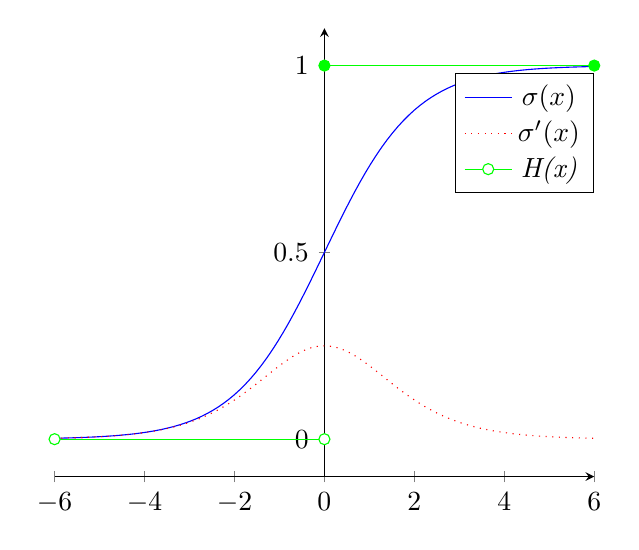
\begin{tikzpicture}[declare function={sigma(\x)=1/(1+exp(-\x));
sigmap(\x)=sigma(\x)*(1-sigma(\x));}]
\begin{axis}%
[
    % grid=major,     
    xmin=-6,
    xmax=6,
    axis x line=bottom,
    ytick={0,.5,1},
    ymax=1.1,
    ymin=-0.1,
    axis y line=middle,
    samples=100,
    domain=-6:6,
    legend style={at={(1,0.9)}}     
]
    \addplot[blue,mark=none]   (x,{sigma(x)});
    \addplot[red,dotted,mark=none]   (x,{sigmap(x)});
    % \addplot[green,mark=none] {(-6, 0), (-0.2, 0), (0.2, 1), (6, 1)};
    \addplot[green, mark=*, mark options={fill=white}, samples at={-6, 0}] {0};
    \addplot[green, mark=*, samples at={0, 6}] {1};
    \legend{$\sigma(x)$,$\sigma'(x)$, $\textit{H(x)}$}
\end{axis}
\end{tikzpicture}
}
      \label{fig:sigmoid function and its derivative}
      \caption{Plot of the sigmoid function, its first derivative and
        the Heaviside step function.}
\end{figure}

For very negative and very positive values of the inputs, the sigmoid approximates
the behaviour of the step function, while for inputs around a neighborhood of 0
it differs by offering a smooth transition between 0 and 1 as an output. It also
is a differentiable function.
This properties allows an approximation of the output when the weights and
biases change slightly as:
\begin{equation*}
  \Delta_{\text{output}} \approx \sum_j\frac{\partial{\text{output}}}{\partial w_j} \Delta w_j + \frac{\partial{\text{output}}}{\partial b}\Delta b
\end{equation*}
This provides an estimation of how small changes in the biases and weights
will affect the output of the sigmoid neuron, making choices for their values
easy to calculate. 

As stated before, all of the computations that take place on a neuron
can be represented in a compact matrix form, as shown in \fref{fig:nn_activation}.
\begin{figure}[!h]
  \centering
  % % \documentclass[tikz]{standalone}
% \usepackage{tikz}
    \usetikzlibrary{positioning}

\tikzset{basic/.style={draw,fill=blue!50!green!20,text width=1em,text badly centered}}
\tikzset{input/.style={basic,circle}}
\tikzset{weights/.style={basic,rectangle}}
\tikzset{functions/.style={basic,circle,fill=blue!10}}

% \begin{document}
    \begin{tikzpicture}
        \node[functions] (center) {};
        \node[below of=center,font=\scriptsize,text width=4em] {Activation function};
        \draw[thick] (0.5em,0.5em) -- (0,0.5em) -- (0,-0.5em) -- (-0.5em,-0.5em);
        \draw (0em,0.75em) -- (0em,-0.75em);
        \draw (0.75em,0em) -- (-0.75em,0em);
        \node[right of=center] (right) {};
            \path[draw,->] (center) -- (right);
        \node[functions,left=3em of center] (left) {$\sum$};
            \path[draw,->] (left) -- (center);
        \node[weights,left=3em of left] (2) {$w_2$} -- (2) node[input,left of=2] (l2) {$x_2$};
            \path[draw,->] (l2) -- (2);
            \path[draw,->] (2) -- (left);
        \node[below of=2] (dots) {$\vdots$} -- (dots) node[left of=dots] (ldots) {$\vdots$};
        \node[weights,below of=dots] (n) {$w_n$} -- (n) node[input,left of=n] (ln) {$x_n$};
            \path[draw,->] (ln) -- (n);
            \path[draw,->] (n) -- (left);
        \node[weights,above of=2] (1) {$w_1$} -- (1) node[input,left of=1] (l1) {$x_1$};
            \path[draw,->] (l1) -- (1);
            \path[draw,->] (1) -- (left);
        \node[weights,above of=1] (0) {$w_0$} -- (0) node[input,left of=0] (l0) {$1$};
            \path[draw,->] (l0) -- (0);
            \path[draw,->] (0) -- (left);
        \node[below of=ln,font=\scriptsize] {inputs};
        \node[below of=n,font=\scriptsize] {weights};
    \end{tikzpicture}
% \end{document}
  \scalebox{1}{
\tikzset{>=latex} % for LaTeX arrow head
\colorlet{myred}{red!80!black}
\colorlet{myblue}{blue!80!black}
\colorlet{mygreen}{green!60!black}
\colorlet{myorange}{orange!70!red!60!black}
\colorlet{mydarkred}{red!30!black}
\colorlet{mydarkblue}{blue!40!black}
\colorlet{mydarkgreen}{green!30!black}
\tikzstyle{node}=[thick,circle,draw=myblue,minimum size=22,inner sep=0.5,outer sep=0.6]
\tikzstyle{node in}=[node,green!20!black,draw=mygreen!30!black,fill=mygreen!25]
\tikzstyle{node hidden}=[node,blue!20!black,draw=myblue!30!black,fill=myblue!20]
\tikzstyle{node convol}=[node,orange!20!black,draw=myorange!30!black,fill=myorange!20]
\tikzstyle{node out}=[node,red!20!black,draw=myred!30!black,fill=myred!20]
\tikzstyle{connect}=[thick,mydarkblue] %,line cap=round
\tikzstyle{connect arrow}=[-{Latex[length=4,width=3.5]},thick,mydarkblue,shorten <=0.5,shorten >=1]
\tikzset{ % node styles, numbered for easy mapping with \nstyle
  node 1/.style={node in},
  node 2/.style={node hidden},
  node 3/.style={node out},
}
\def\nstyle{int(\lay<\Nnodlen?min(2,\lay):3)} % map layer number onto 1, 2, or 3



\begin{tikzpicture}[x=2.7cm,y=1.6cm]
  \message{^^JNeural network activation}
  \def\NI{5} % number of nodes in input layers
  \def\NO{4} % number of nodes in output layers
  \def\yshift{0.4} % shift last node for dots
  
  % INPUT LAYER
  \foreach \i [evaluate={\c=int(\i==\NI); \y=\NI/2-\i-\c*\yshift; \index=(\i<\NI?int(\i):"n");}]
              in {1,...,\NI}{ % loop over nodes
    \node[node in,outer sep=0.6] (NI-\i) at (0,\y) {$a_{\index}^{(0)}$};
  }
  
  % OUTPUT LAYER
  \foreach \i [evaluate={\c=int(\i==\NO); \y=\NO/2-\i-\c*\yshift; \index=(\i<\NO?int(\i):"m");}]
    in {\NO,...,1}{ % loop over nodes
    \ifnum\i=1 % high-lighted node
      \node[node hidden]
        (NO-\i) at (1,\y) {$a_{\index}^{(1)}$};
      \foreach \j [evaluate={\index=(\j<\NI?int(\j):"n");}] in {1,...,\NI}{ % loop over nodes in previous layer
        \draw[connect,white,line width=1.2] (NI-\j) -- (NO-\i);
        \draw[connect] (NI-\j) -- (NO-\i)
          node[pos=0.50] {\contour{white}{$w_{1,\index}$}};
      }
    \else % other light-colored nodes
      \node[node,blue!20!black!80,draw=myblue!20,fill=myblue!5]
        (NO-\i) at (1,\y) {$a_{\index}^{(1)}$};
      \foreach \j in {1,...,\NI}{ % loop over nodes in previous layer
        %\draw[connect,white,line width=1.2] (NI-\j) -- (NO-\i);
        \draw[connect,myblue!20] (NI-\j) -- (NO-\i);
      }
    \fi
  }
  
  % DOTS
  \path (NI-\NI) --++ (0,1+\yshift) node[midway,scale=1.2] {$\vdots$};
  \path (NO-\NO) --++ (0,1+\yshift) node[midway,scale=1.2] {$\vdots$};
  
  % EQUATIONS
  \def\agr#1{{\color{mydarkgreen}a_{#1}^{(0)}}}
  \node[below=17,right=11,mydarkblue,scale=0.95] at (NO-1)
    {$\begin{aligned} %\underset{\text{bias}}{b_1}
       &= \color{mydarkred}\sigma\left( \color{black}
            w_{1,1}\agr{1} + w_{1,2}\agr{2} + \ldots + w_{1,n}\agr{n} + b_1^{(0)}
          \color{mydarkred}\right)\\
       &= \color{mydarkred}\sigma\left( \color{black}
            \sum_{i=1}^{n} w_{1,i}\agr{i} + b_1^{(0)}
           \color{mydarkred}\right)
     \end{aligned}$};
  \node[right,scale=0.9] at (1.3,-1.3)
    {$\begin{aligned}
      {\color{mydarkblue}
      \begin{pmatrix}
        a_{1}^{(1)} \\[0.3em]
        a_{2}^{(1)} \\
        \vdots \\
        a_{m}^{(1)}
      \end{pmatrix}}
      &=
      \color{mydarkred}\sigma\left[ \color{black}
      \begin{pmatrix}
        w_{1,1} & w_{1,2} & \ldots & w_{1,n} \\
        w_{2,1} & w_{2,2} & \ldots & w_{2,n} \\
        \vdots  & \vdots  & \ddots & \vdots  \\
        w_{m,1} & w_{m,2} & \ldots & w_{m,n}
      \end{pmatrix}
      {\color{mydarkgreen}
      \begin{pmatrix}
        a_{1}^{(0)} \\[0.3em]
        a_{2}^{(0)} \\
        \vdots \\
        a_{n}^{(0)}
      \end{pmatrix}}
      +
      \begin{pmatrix}
        b_{1}^{(0)} \\[0.3em]
        b_{2}^{(0)} \\
        \vdots \\
        b_{m}^{(0)}
      \end{pmatrix}
      \color{mydarkred}\right]\\[0.5em]
      {\color{mydarkblue}a^{(1)}}
      &= \color{mydarkred}\sigma\left( \color{black}
           \mathbf{W}^{(0)} {\color{mydarkgreen}a^{(0)}}+\mathbf{b}^{(0)}
         \color{mydarkred}\right)
         %\color{black},\quad \mathbf{W}^{(0)} \in \mathbb{R}^{m\times n}
    \end{aligned}$};
  
\end{tikzpicture}
}
  \caption{Input to a single neuron in a feedforward network. Here
    $\sigma$ represents the activation function (a sigmoid function in
    this case) and the exponents represent layers. The activation of a
    layer can be conveniently represented in matrix form. Biases are added
    to the input of the node.}
  \label{fig:nn_activation}
\end{figure}

\newpage
\subsection*{Learning}

Before defining how training works for a neural network, it is
imperative to describe an algorithm of quantifying far from the
target output the network is with its current biases and weights.
This algorithm is the \textit{cost function} described in \sref{sec:gradient_descent}.

If for all inputs in a vector $\bm{x}$ the desired output is known and is
the output of some function $f^{*}(\bm{x}) ~\text{or}~ y(\bm{x})$ and the
cost function can be defined as:
% \newpage
\begin{equation}
  \label{eq:cost_func_simple}
  C(\bm{w}, \bm{b}) = \frac{1}{2n} \sum_x ||y(\bm{x}) - \bm{a}||^2
\end{equation}

In this equation, $\bm{w}~\text{and}~\bm{b}$ are the weights and biases
of the network respectively and $\bm{a}$ is a vector of the outputs when
$\bm{x}$ is the input.

This cost function is also known as \textit{quadratic} or \textit{mean
  squared error (MSE)} and it is one of the most commonly used loss
functions. 
The goal of training is to minimize this function, and to achieve this
gradient descent and variations of this method are used.

Applying gradient descent to \eref{eq:cost_func_simple} yields:
\begin{equation}
  \label{eq:cost_func_grad}
  \nabla C = \frac{1}{n} \sum_x\nabla C_x
\end{equation}
where $x$ are the training samples.

\subsubsection*{Stochastic Gradient Descent (SGD)}
One of the most common variations is \textit{Stochastic Gradient
Descent (SGD)}. As training sets get larger, they become
computationally expensive especially considering that in
\eref{eq:cost_func_simple}, the total cost function $C =
\frac{1}{n}\sum_x C_x$, averaging the costs of each training sample.
The gradient of this function requires the computation of each $\nabla
C_x$ for each sample and then averaging them as $\nabla C =
\frac{1}{n}\sum_x\nabla C_x$ which can be prohibitive timewise.

SGD offers a solution to this problem, by drastically simplifying
the above process; instead of finding the exact value of $\nabla C$
, it estimates its value by randomly picking one sample \cite{article:bottou}.
This stochastic approximation adds noise, but it has been proven to
almost ensure convergence under mild conditions \cite{book:robbins}.

\begin{figure}[!h]
  \centering
  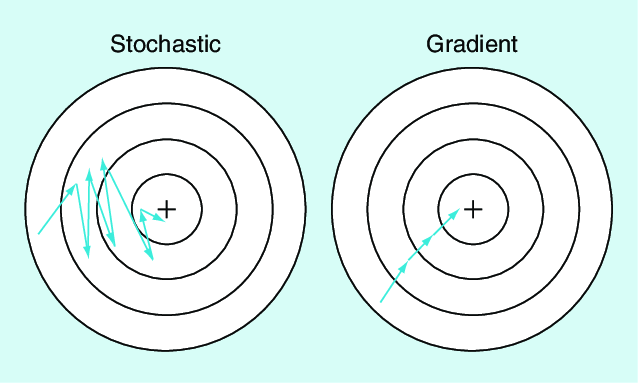
\includegraphics[width=.8\textwidth]{Figures/chap_nn/gradient_stoch.png}
  \caption{Noisy convergence of SGD compared to non-stochastic. Image
source \cite{article:image_gradient}.}
  \label{fig:gradient_descent_noisy}
\end{figure}

A smoother convergence by choosing a small number $m$ of samples which
is called a \textbf{mini-batch} and is the method most commonly used as
it offers a compromise between speed and smoothness of convergence.
In this case, \eref{eq:cost_func_grad} becomes:
\begin{equation}
  \label{eq:cost_func_stoch}
  \nabla C \approx \frac{1}{m} \sum_{i=1}^m \nabla C_{X_j}
\end{equation}

\subsubsection*{Training rules}

We can then define a training rule for the network in terms of
weights and biases and using the gradient of the cost function.
Applying SGD on \eref{eq:cost_func_simple} provides
the values of weights $w_k$  and biases $b_l$ that minimizes it. An update rule
for them can now be defined in terms of the cost function:
\begin{align}
  w_k \rightarrow w^{'}_k &= w_k - \frac{\eta}{m}\sum_j \frac{\partial C_{x_j}}{\partial w_k} \nonumber \\
  b_l \rightarrow b^{'}_l &= b_l - \frac{\eta}{m}\sum_j \frac{\partial C_{x_j}}{\partial b_l}
  \label{eq:update_w_b}
\end{align}

where $\eta$ is a small positive value, the \textbf{learning rate}. 

Having described the above, the process of training the NN can be summarized as:
\begin{enumerate}
\item The SGD is calculated for a random set number of training samples, the mini-batch.
\item Weights and biases are updated based on \eref{eq:yolo}.
\item The previous two steps are repeated until the training samples are exhausted.
\item When all samples are exhausted, the training \textbf{epoch} is complete, and the
  process starts again from the first step.
\item Training is usually said to be complete, when the value of  the cost function
  is below a set threshold. The NN is now considered trained.
\end{enumerate}

\subsection{Backpropagation}

Backpropagation is a method of computing the gradient of the loss function
with respect to all the weights and biases of the network, based on single
training examples, in contrast to more naive methods which compute the gradient
on each weight or bias individually.

Even though these days the term \textit{backpropagation} is sometimes
used colloquially to refer to the whole process of the learning algorithm,
strictly it is just an algorithm to compute the gradient, while SGD can be
used for the training itself \cite{book:Goodfellow}.

Historically, this method has been rediscovered multiple times, as early
as 1960 \cite{article:SCHMID} with its first implementation as
software in 1970 \cite[p.~229]{book:Goodfellow}, albeit as a method
for automatic differentation with no mention to neural networks. In
1974, Werbos proposed its usage in training neural
networks\cite{book:WerbosBackprop}, but it was not until 1986 when
\citet*{article:backprop} published their seminal paper ``Learning
representations by back-propagating errors'' which experimentally
showed that backpropagation can be used to train deep neural networks
faster than any existing technique up to that point.


Ultimately the goal of backpropagation is to compute the partial
derivatives $\frac{\partial C_X}{\partial w^l_{jk}} ~\text{and}~ \frac{\partial
  C_X}{\partial b^l_{j}}$ --- the partial derivates of the cost function
 with respect to weights and biases in the network.


\subsubsection*{Matrix Notation}

Before introducing the equations of backpropagation, it is
important to present a matrix notation for quantities in a
network which are used widely and unambigiuous. Consider the
equations presented in \fref{fig:nn_activation}. For a network
with $L$ layers, the connection of the $k^{th}$ neuron in the
$(l-1)^{th}$ layer with $j^{th}$ node in $l^{th}$ layer can be
written as $w_{jk}^l$. In a similar fashion, the bias of the
$j^{th}$ node in the $l^{th}$ layer can be represented as $b^l_j$
and the \textit{activation}\footnote{The activation of a neuron
  simply refers to the output of the activation function, taking as
  input the weighted sum of the inputs and the bias $a' = \sigma(wa +
  b)$
} of the same node is $a_j^l$. With this representations declared
it is possible to define the matrix representation of a layer $l$ as:
\begin{equation}
  \label{eq:layer}
  \bm{a^l} = \sigma(\bm{w^l} \bm{a^{l-1}} + \bm{b^l})
\end{equation}

where $\sigma$ is the activation function. At this point the
intermediate quantity $\bm{z^l} = \bm{w^la^{l-1}} + \bm{b^l}
\rightarrow \bm{a^l} = \sigma(\bm{z^l})$ commonly called the
\textit{weighted input} is worth declaring.

\subsubsection*{Fundamentals of Backpropagation}

Backpropagation has two special requirements for the
cost function. The first is that it must be able to be
written as an average $C = \frac{1}{n} \sum_XC_X$ of the
cost functions of individual training samples $x$. This
ensures that after computing the partial derivatives
$\frac{\partial C_X}{\partial w} \text{and} \frac{\partial C_X}{partial b}$
over the training set, it is possible to calculate 
$\frac{\partial C}{\partial w} \text{and} \frac{\partial C}{\partial b}$
by averaging over the set.

The second requirement is that the cost function $C$ can be
written as a function of the outputs of the NN. For example,
the MSE cost function described in \eref{eq:cost_func_simple}
for a single training example can be written as
\begin{equation}
  \label{eq:backprop_mse}
  C = \frac{1}{2}||\bm{y} - \bm{a^L}|| = \frac{1}{2}\sum_j(y_j - a^L_j)^2
\end{equation}

which in fact can be regarded a function of the outputs $\bm{a^L}$ alone,
as the training examples $y(x)$ have fixed values. Note that $L$ denotes the
number of layers in the networks.

\subsubsection*{Equations of backpropagation}

Before declaring the fundamental equations of backpropagation,
an important intermediate quantity called the \textbf{error} $\delta_j^l$
must be declared. In a neuron $j$, during activation, a small quantity $\Delta z_j^l$
is added as input and the neuron outputs $\sigma (z^l_j + \Delta z_j^l)$.
This error is propagated through the network and finally
the overall cost changes by $\frac{\partial C}{\partial z_j^l}\Delta z_j^l$.
The error can the be defined as:
\begin{equation}
  \label{eq:error_nn}
  \delta_j^l \equiv \frac{\partial C}{\partial z_j^l}
\end{equation}


The fundamental equations which govern the backpropagation process
are described below.
\begin{enumerate}
\item
  The first equation describes the error in the
  \textbf{output layer}:
  \begin{equation}
    \delta^L_j = \frac{\partial C}{\partial a_j^L} \sigma'(z_j^L)
  \end{equation}
  or equivalently in matrix form:
  \begin{equation}
    \label{eq:error_output}
    \delta^L = \bm{\nabla_a C} \odot \sigma' (\bm{z^L})
  \end{equation}
\item
  An equation for the error in terms of the error in the
  \textbf{next layer}:
  \begin{equation}
    \label{eq:error_layer}
    \delta^l = ((\bm{w^{l+1}})^T\bm{\delta^{l+1}})\odot \sigma'(\bm{z^l})
  \end{equation}
  This equation is convenient as it propagates the error backwards
  in the network. Knowning the error in the $(l+1)^{th}$ layer and
  by transposing the weight matrix the error can then move backwards
  through the activation function in layer $l$. This process can be
  repeated all the way back.
\item
  An equation describing the rate of change of the cost with respect to \textbf{biases}
  in the network:
  \begin{equation}
    \label{eq:error_bias}
    \frac{\partial C}{\partial b_j^l} = \delta^l_j \xrightarrow{\ref{eq:error_layer},~~ \ref{eq:error_output}} \frac{\partial C}{\partial b} = \delta 
  \end{equation}
\item
  An equation describing the rate of change of the cost with respect
  to \textbf{weights} in the network:
  \begin{equation}
    \label{eq:error_cost}
    \frac{\partial C}{\partial w_{jk}^l} = a^{l-1}_k\delta^l_j
  \end{equation}
  
\end{enumerate}

Finally, \eref{eq:error_bias} and \eref{eq:error_cost} have been
derived and can now be used in SGD or other learning algorithms.

The importance of backpropagation as a method arises from the fact that it is
possible to compute all the partial derivatives of the cost function
with just one forward and one backward pass through the network. Before
its emergence, training a network required computing these derivatives
for each weight and bias individually, which was prohibitively time consuming
for larger networks.


\subsubsection*{Learning algorithm using backpropagation}

The backpropagation algorithm can be represented in pseudocode
as shown below.


\begin{algorithm}
\caption{Backpropagation Algorithm}
\label{alg:Backprop}
\DontPrintSemicolon
\KwData{$\bm{x}$ the activation of the input layer $\bm{a^1}$}
\KwResult{The gradient of $C$ in terms of $\frac{\partial C}{\partial w_{jk}^l} = a^{l-1}_k\delta_j^l ~\text{and} ~ \frac{\partial C}{\partial b_j^l} = \delta_j^l$}
\Begin{
  % layers = $1, 2, 3, ... L$\;
  $layers \gets [2, 3, ... L ]$\;
  \tcp{Feedforward pass}
  \For {l in layers}{
    $z^l \gets w^la^{l-1} + b^l$\;
    $a^l \gets \sigma(z^l)$\;
  }
  \tcp{Output: Error vector}
  $\bm{\delta^l} \gets \nabla_a \bm{C} \odot \bm{\sigma'(z^L)}$ \;
  \tcp{Backpropagate the error}
  $layers\_reverse \gets [L-1, L-2, ... 2]$\;
  \For {l in layers\_reverse}{
    $ \bm{\delta^l} \gets ((\bm{(w^{l+1})^T\delta^{l+1}}) \odot \bm{\sigma'(z^l)}$\;
  }
  
  \tcp{Output}
  $\frac{\partial C}{\partial w_{jk}^l} \gets a^{l-1}_k\delta_j^l$\;
  $\frac{\partial C}{\partial b_j^l} \gets \delta_j^l$\;
}
\end{algorithm}

Consequently, combining backpropagation and a learning algorithm
such as a SGD, it is possible to train a network. For instance,
in a SGD with $m$ mini-batches case, the training rules, as described
in \eref{eq:update_w_b}, can be represented with the following pseudo-code:


\begin{algorithm}
\caption{Training Rules using SGD with backpropagation}
\label{alg:Training_Backprop}
\DontPrintSemicolon
\KwData{Sets of training examples}
\KwResult{Updated weights and biases based on gradient descent of the cost function}
\Begin{
  % layers = $1, 2, 3, ... L$\;
  $a^{x, l} \gets \text{set the activation for each sample}$\;
  \tcp{Pass the activation to the backpropagation from \Aref{alg:Backprop}
    and get the error as output}
  $\delta^{x,l} = ((w^{l+1})^T\delta^{x,l+1})\odot \sigma'(z^{x,l})$\;
  \tcp{Gradient Descent and updates for weights and biases}
  $layers\_reverse \gets [L-1, L-2, ... 2]$\;
  \For {l in layers\_reverse}{
  $ w^{l'} \gets w^l - \frac{\eta}{m}\sum_x\delta^{x,l}(a^{x,l-1})^T$\;
  $b^{l'} \gets b^l - \frac{\eta}{m}\sum_x\delta^{x,l}$\;
  }
}
\end{algorithm}

\clearpage
\subsection{Common ANN Architectures}

So far, the models discussed were simple perceptrons and multi-layer
perceptrons (MLPs), networks which are fully connected --- each neuron
in a layer is connected to all the neurons of the next layer (i.e. see
\fref{fig:simple_nn_demo}). This architecture does not take into
account that data used as input might carry some spatial structure, as
in the case of image recognition and computer vision.  In this
section, convolutional neural networks will be introduced briefly,
which take into account the spatially local input patterns of some
datasets, while at the same time reducing the number of free parameters
allowing for deeper networks. While the origin of these types of
networks can be traced to 1970, they were first established as a concept
by LeCun in the paper ``Gradient-based learning applied to document
recognition'' from \citet{article:lecun1998}.

\subsubsection{Convolutional Neural Networks (CNNs)}

As mentioned before, CNNs take advantage of the spatial structure that
some types of data have. For instance an image has a grid-topology,
which is ignored in the case of simple or deep MLPs and as a consequence it
inhibits learning by treating pixels which are spatially far, in the same
manner. CNNs architecture solve this problem by taking into account
the spatial characteristics of their input data. The basic concepts of
CNNs are \textit{local receptive fields, shared weights} and \textit{pooling}.
In this context, the input layer is considered to be 2-dimensional structure
typically a square.

\textbf{Local receptive fields}

Each neuron of the hidden layer is connected to a
small region of the input layer, typically a small square, which
is called the \textit{local receptive field} of the hidden neuron.
Each of these connections has a trainable weight, and the neuron has a bias.
The region is slid across the input layer, passing values to the hidden layer.

\textbf{Shared weights and biases}

All of the hidden neurons share the same weights and biases; with the activation
of the i, $k$th neuron begin:
\begin{equation}
  \label{eq:cnn_activation}
  \sigma \bigg(b + \sum_{l=0}^{r_x}\sum_{m=0}^{r_y}w_{l,m}a_{j+l,k+m}\bigg)
\end{equation}

where $\sigma$ represents the neural activation function, $a_{x,y}$
are the activations of the input at those coordinates and $r_x, r_y$
are the dimensions of the receptive field.

Sharing weights and biases allows for features to be detected
from input data, in conjuction with their spatial coordinates.
For this reason, the mapping of the input layer to the hidden
layer is called a \textit{feature map}, and the shared weights
and biases are often called a \textit{kernel} or \textit{filter}.
Typically, CNNs have several of these feature maps, one for each
feature they are configured (or learn) to detect.

\begin{figure}[H]
  \centering
  \usetikzlibrary{decorations.pathreplacing}
% \begin{SCfigure}[2\sidecaptionrelwidth][t]
% 	\centering
	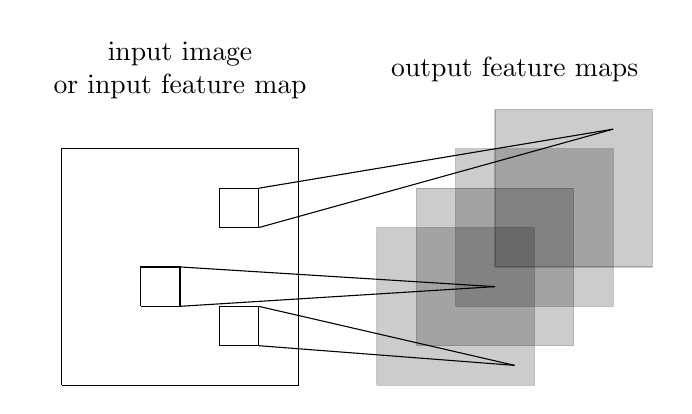
\begin{tikzpicture}
		\node at (1.5,4){\begin{tabular}{c}input image\\or input feature map\end{tabular}};
	
		\draw (0,0) -- (3,0) -- (3,3) -- (0,3) -- (0,0);
		
		\draw (2,2) -- (2.5,2) -- (2.5,2.5) -- (2,2.5) -- (2,2);
		\draw (2,0.5) -- (2.5,0.5) -- (2.5,1) -- (2,1) -- (2,0.5);
		\draw (1,1) -- (1.5,1) -- (1.5,1.5) -- (1,1.5) -- (1,1);
		
		\draw (2.5,2) -- (7,3.25);
		\draw (2.5,2.5) -- (7,3.25);
 
		\draw (2.5,1) -- (5.75,0.25);
		\draw (2.5,0.5) -- (5.75,0.25);
		
		\draw (1.5,1.5) -- (5.5,1.25);
		\draw (1.5,1) -- (5.5,1.25);
		
		\node at (5.75,4){\begin{tabular}{c}output feature maps\end{tabular}};
		
		\draw[fill=black,opacity=0.2,draw=black] (5.5,1.5) -- (7.5,1.5) -- (7.5,3.5) -- (5.5,3.5) -- (5.5,1.5);
		\draw[fill=black,opacity=0.2,draw=black] (5,1) -- (7,1) -- (7,3) -- (5,3) -- (5,1);
		\draw[fill=black,opacity=0.2,draw=black] (4.5,0.5) -- (6.5,0.5) -- (6.5,2.5) -- (4.5,2.5) -- (4.5,0.5);
		\draw[fill=black,opacity=0.2,draw=black] (4,0) -- (6,0) -- (6,2) -- (4,2) -- (4,0);
	\end{tikzpicture}
	% \caption[Illustration of a convolutional layer.]{Illustration of a single convolutional layer. If layer $l$ is a convolutional layer, the input image (if $l = 1$) or a feature map of the previous layer is convolved by different filters to yield the output feature maps of layer $l$.}
	% \label{fig:convolutional-layer}
% \end{SCfigure}
  \caption{Illustration of a convolutional layer with multiple feature maps.}
  \label{fig:feature_maps}
\end{figure}

\textbf{Pooling Layers} Pooling layers are typically
used immediately after the convolutional (hidden) layers.  It reduces
the dimensions of clusters of neuros into a signle neuron in the next
layer. The two most common pooling procedures are max-pooling which
outputs the maximum activation from the pooling region and the average
pooling which outputs the average value of the activations.

\begin{figure}[H]
  \centering
  \usetikzlibrary{decorations.pathreplacing}

	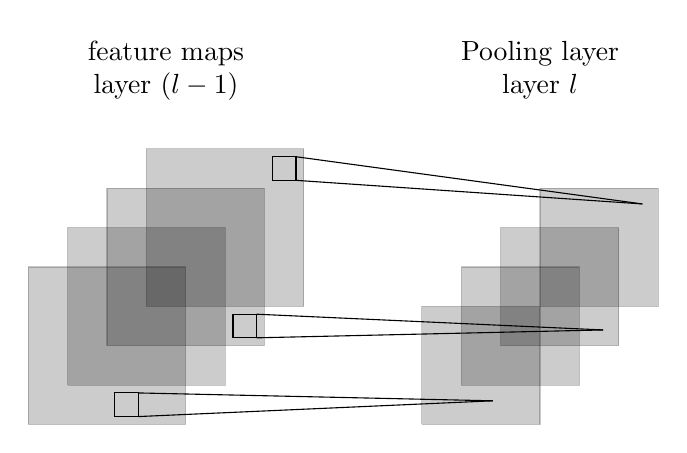
\begin{tikzpicture}
		\node at (1.75,4.5){\begin{tabular}{c}feature maps\\layer $(l-1)$\end{tabular}};
		
		\draw[fill=black,opacity=0.2,draw=black] (1.5,1.5) -- (3.5,1.5) -- (3.5,3.5) -- (1.5,3.5) -- (1.5,1.5);
		\draw[fill=black,opacity=0.2,draw=black] (1,1) -- (3,1) -- (3,3) -- (1,3) -- (1,1);
		\draw[fill=black,opacity=0.2,draw=black] (0.5,0.5) -- (2.5,0.5) -- (2.5,2.5) -- (0.5,2.5) -- (0.5,0.5);
		\draw[fill=black,opacity=0.2,draw=black] (0,0) -- (2,0) -- (2,2) -- (0,2) -- (0,0);
		
		\draw (3.1,3.1) -- (3.4,3.1) -- (3.4,3.4) -- (3.1,3.4) -- (3.1,3.1);
		\draw (2.6,1.1) -- (2.9,1.1) -- (2.9,1.4) -- (2.6,1.4) -- (2.6,1.1);
		\draw (1.1,0.1) -- (1.4,0.1) -- (1.4,0.4) -- (1.1,0.4) -- (1.1,0.1);
		
		\draw (3.4,3.4) -- (7.8,2.8);
		\draw (3.4,3.1) -- (7.8,2.8);
		
		\draw (2.9,1.4) -- (7.3,1.2);
		\draw (2.9,1.1) -- (7.3,1.2);
		
		\draw (1.4,0.4) -- (5.9,0.3);
		\draw (1.4,0.1) -- (5.9,0.3);
		
		\node at (6.5,4.5){\begin{tabular}{c}Pooling layer\\layer $l$\end{tabular}};
		
		\draw[fill=black,opacity=0.2,draw=black] (6.5,1.5) -- (8,1.5) -- (8,3) -- (6.5,3) -- (6.5,1.5);
		\draw[fill=black,opacity=0.2,draw=black] (6,1) -- (7.5,1) -- (7.5,2.5) -- (6,2.5) -- (6,1);
		\draw[fill=black,opacity=0.2,draw=black] (5.5,0.5) -- (7,0.5) -- (7,2) -- (5.5,2) -- (5.5,0.5);
		\draw[fill=black,opacity=0.2,draw=black] (5,0) -- (6.5,0) -- (6.5,1.5) -- (5,1.5) -- (5,0);
	\end{tikzpicture}
  \caption{Illustration of the pooling layer following the feature maps}
  \label{fig:pooling}
\end{figure} % Review of the Literature

\chapter{Notation \& Fundamentals} \label{methodology}
 % Fundamentals

\chapter{Basic Principles and Implementation Framework for an [Problem to be Solved]} \label{framework}
 % Framework

\chapter{Implementation and Core Components of [Platform Title]} \label{platform}
 % Platform

\chapter{Experimentation \& Validation} \label{experimentationANDresults}
 % Experimentation

\chapter{Conclusions \& Future Work} \label{conclusions}
 % Results and Discussion

%\input{Chapters/Chapter7} % Conclusion

%% ----------------------------------------------------------------
% Now begin the Appendices, including them as separate files

\addtocontents{toc}{\vspace{2em}} % Add a gap in the Contents, for aesthetics

\appendix % Cue to tell LaTeX that the following 'chapters' are Appendices

% \chapter{Example Appendix} \label{math}
 
% Example appendices

\addtocontents{toc}{\vspace{2em}}  % Add a gap in the Contents, for aesthetics
\backmatter % End the book's numbering; backpage

%% ----------------------------------------------------------------
\label{Bibliography}
\lhead{\emph{Bibliography}}  % Change the left side page header to "Bibliography"
% \bibliographystyle{ACM-Reference-Format}
\bibliographystyle{unsrtnat}  % Use the "unsrtnat" BibTeX style for formatting the Bibliography
\bibliography{Bibliography}  % The references (bibliography) information are stored in the file named "Bibliography.bib"

\end{document}  % The End
%% ----------------------------------------------------------------
